\def\VCDate{2016/02/12}\def\VCVersion{(Current)}
\documentclass[11pt]{article}
\usepackage[screen]{geometry}
\usepackage{ProofPower,graphicx, color}
\usepackage{amsmath, amssymb}
\begin{document}

\title{CS113 Lab:1}
\author{Saw Thinkar Nay Htoo}
\maketitle
\section*{Purpose}
To explore the tools to create documents with math symbols combined with programming and to learn about logic connectives used in propositional calculus. \footnote{lab1 second draft}

\begin{itemize}

\item
The truth table value of $p \land q$.(Conjunction)\\
\input and.tex
\clearpage

\item
The truth table value of $p \lor q$.(Disjunction)\\
\input or.tex


\item
The truth table value of $p \oplus q$.(Exclusive or)\footnote{Unnecessary "r" is removed from the truth table.}\\
\input xor.tex

\clearpage

\item
The truth table value of $\sim p$ and $\sim q$.(Negation)\footnote{Negation signs are changed from $\neg$ to $\sim$.}\\
\input not1.tex
\input not2.tex

\end{itemize}

\noindent{ \color{red} \rule{\linewidth} {0.5mm} }
\clearpage

\section*{SML codes for conjuntion, disjunction, exclusive or and negation}
SML code for conjunction. When the two values are True, the result is True. Otherwise the rest of the results are False.\footnote{Output results for SML codes are added and function names are changed to long form to reduce confusion.}
\begin{GFT}{SML}
\+datatype Bool = F | T;\\
\+fun conjunction(F,x) = F\\
\+ | conjunction(T,x) = x;\\
\+conjunction(F,F);\\
\+conjunction(T,F);\\
\+conjunction(F,T);\\
\+conjunction(T,T);\\
\+val truth\_values = [(F,F),(F,T),(T,F),(T,T)];\\
\+map conjunction truth\_values;\\
\end{GFT}
\includegraphics[scale = 0.6]{con.png}
\clearpage

SML code for disjunction. When the two values are False, the output is False. The rest of the results are True.
\begin{GFT}{SML}
\+datatype Bool = F | T;\\
\+fun disjunction(F,F) = F\\
\+| disjunction(T,x) = T\\
\+| disjunction(x,T) = T;\\
\+disjunction(F,F);\\
\+disjunction(T,F);\\
\+disjunction(F,T);\\
\+disjunction(T,T);\\
\+val truth\_values = [(F,F),(F,T),(T,F),(T,T)];\\
\+map disjunction truth\_values;\\
\end{GFT}
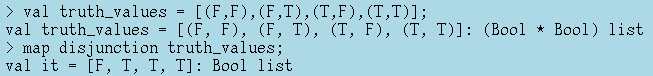
\includegraphics[scale=0.6]{dis.png}
\clearpage

SML code for exclusive or. When the values are the same, the output is False. When the values are different, the output is True.\\
\begin{GFT}{SML}
\+datatype Bool = F | T;\\
\+fun exclusive\_or (T,T) = F\\
\+ | exclusive\_or (F,F) = F\\
\+ | exclusive\_or (x,y) = T;\\
\+exclusive\_or(F,F);\\
\+exclusive\_or(T,F);\\
\+exclusive\_or(F,T);\\
\+exclusive\_or(T,T);\\
\+val truth\_values = [(F,F),(F,T),(T,F),(T,T)];\\
\+map exclusive\_or truth\_values;\\
\end{GFT}
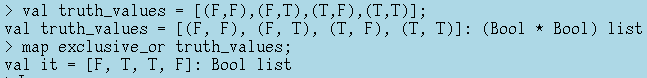
\includegraphics[scale=0.6]{xor.png}
\clearpage

SML code for negation. The values are reversed.\\
\begin{GFT}{SML}
\+datatype Bool = F | T;\\
\+fun negation T = F\\
\+ | negation F = T;\\
\+negation (T);\\
\+negation (F);\\
\+val truth\_values = [F,T];\\
\+map negation truth\_values;\\
\end{GFT}
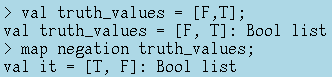
\includegraphics[scale=0.6]{neg.png}\\
\noindent{ \color{red} \rule{\linewidth} {0.5mm} }
\clearpage

\clearpage

\section*{Problem 1.18}
Show that $p \oplus q \equiv (p \lor q) \land \sim (p \land q)$. \footnote{Negation signs are changed from $\neg$ to $\sim$.}\\
\begin{enumerate}
\item 
Left hand side 
\input xor2.tex 

\item
Right hand side 
\input test1.tex 

\item
LHS = RHS (Hence shown)
\end{enumerate} 
\clearpage

This is the result created by inputting the entire equation into the truth table generator.\footnote{Negation signs are changed from $\neg$ to $\sim$. Table is created again with details.}
\input 118.tex

section*{SML code for 1.18}\footnote{Function names are changed to long form to help readers not to be confused. }
\begin{GFT}{SML}
\+datatype Bool = F | T;\\
\+fun negation T = F\\
\+ | negation F = T;\\
\+fun exclusive\_or (T,T) = F\\
\+ | exclusive\_or (F,F) = F\\
\+ | exclusive\_or (x,y) = T;\\
\+fun disjunction(F,F) = F\\
\+ | disjunction(T,x) = T\\
\+ | disjunction(x,T) = T;\\
\+fun conjunction(F,x) = F\\
\+ | conjunction(T,x) = x;\\
\end{GFT}
\clearpage
conjunction(p,q) is created first since it is most inner function. Then its negation and disjunction(p,q) are built simultaneously. Then both of their results are used for outer most function(conjunction) of the left hand side.\footnote{Explanation added.}\\
For left hand side, "exclusive or" function is operated.\\
\begin{GFT}{SML}
\+conjunction(disjunction(T,F),negation(conjunction(T,F)));\\
\+exclusive\_or(T,F);\\
\+\\
\end{GFT}
Since the result of the both functions are the same as True's, it is concluded that left hand side is equal to right hand side. (Below figure) \\
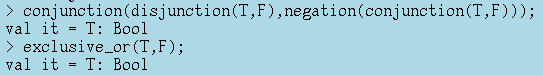
\includegraphics[scale=0.6]{118.png}
\clearpage

\section*{Sample Code and its result by the professor.}
\begin{GFT}{SML}
\+datatype Bool = F | T;\\
\+fun conjunction (F,F) = F\\
\+ | conjunction (F,T) = F\\
\+ | conjunction (T,F) = F\\
\+ | conjunction (T,T) = T;\\
\+val truth\_values = [(F,F),(F,T),(T,F),(T,T)];\\
\+map conjunction truth\_values;\\
\+\\
\end{GFT}
Running above SML code produces this truth table:\footnote{Explanation added.}\\
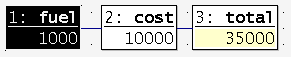
\includegraphics[scale= 0.6]{out1.png}
\begin{GFT}{SML}
\+infix AND;\\
\+fun p AND q = conjunction (p,q);\\
\+T AND F;\\
\end{GFT}
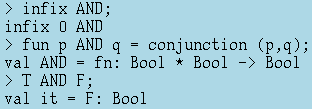
\includegraphics[scale = 0.6]{out2.png}\\
A new function is created using infix AND, thus making the code less confusing and easier to understand. This method is supposed to be used in problem 1.18\\
\clearpage

\section*{Review Questions}
\begin{itemize}

\item
Problem 1.9 \\
Question: Use De Morgan's laws to write the negation for the proposition: "The dollar is at an all-time high and the stock market is at a record low."\\
Answer: The dollar is \textbf{not} at an all-time high \textbf{or} the stock market is \textbf{not} at a record low.\\
Note: This is not the result of the negation: "The dollar is at an all-time \textbf{low} \textbf{or} the stock is at a record \textbf{high}."

\noindent{ \color{red} \rule{\linewidth} {0.5mm} }

\item
Problem 1.10 \\
Question: Assume $x \in \mathbb{R}$. Use De Morgan's laws to write the negation for the proposition: $-5 < x <= 0$.\footnote{Changed to correct symbols by adding delimiters. Explanation for DeMorgan's law added.} \\
Answer:  $x \leq -5$ or $x > 0$ \\
Note: Less than or equal sign is changed to the other side of the equation. Definition of DeMorgan's Law: "The negation of a conjunction is the disjunction of the negations. The negation of a disjunction is the conjunction of the negations." Ref: wikipedia. In this case, as we can see less-than-or-equal signs are changed on both side and "or" is added in between two ranges of values of possible value of x. 

\noindent{ \color{red} \rule{\linewidth} {0.5mm} }
\clearpage

\item
Problem 1.12
Question: Show that the proposition $s = (p \land \sim q) \land (\sim p \lor q)$ is a contradiction. \footnote{Explanation added.} \\
Answer: \textbf{Contradiction}: A compound proposition that has the value F for all possible values of the propositions in it. \\
\input 112.tex \\
\noindent{ \color{red} \rule{\linewidth} {0.5mm} }
\clearpage


\item
Problem 1.13 (c)
Question: Is $(p \oplus q) \land r \equiv (p \land r) \oplus (q \land r)$ ? Justify your answer. \\
Answer:  As we can see the results of the fifth and eighth columns of the table are the same, it is concluded that left hand side is equal to right hand side. \\
\input 113c.tex \\
\noindent{ \color{red} \rule{\linewidth} {0.5mm} }
\clearpage

\item
Problem 1.14 (c)
Question:  $\sim t \equiv$ c and $\sim c \equiv t$, where t is a tautology and c is a contradiction. \\
Answer: \footnote{Definitions added. Tables edited.}\\
\textbf{Tautology}: A compound prosition which is always true, regardless of the truth values of the propositional variables which comprise it.\\
\textbf{Contradiction}: A compound proposition that has the value F for all possible values of the propositions in it. \\
\input 114c1.tex
\input 114c2.tex\\
\noindent{ \color{red} \rule{\linewidth} {0.5mm} }
\clearpage

\item
Problem 1.14 (d) 
Question: $p \lor p \equiv p$ and $p \land p \equiv p$ \\
Answer:
\input 114d1.tex  
\input 114d2.tex \\
\noindent{ \color{red} \rule{\linewidth} {0.5mm} }

\item
Problem 1.20 
Question: Show that $\sim p \land (p \land q)$ is a contradiction. \\
Answer: 
\input 120.tex 
\clearpage
\end{itemize}
\end{document}
